\documentclass[14pt,usenames,dvipsnames]{beamer}
\usepackage[utf8]{inputenc}
\usefonttheme{structurebold}
\usepackage{cabin}
\usepackage[absolute,overlay,showboxes]{textpos}
\usepackage{multimedia}

\usetheme{Madrid}
\usecolortheme{default}

\setbeamertemplate{itemize items}[triangle]
%\setbeamercolor{section number projected}{bg=blue,fg=white}
\setbeamertemplate{section in toc}[ball]
\setbeamertemplate{subsection in toc}[triangle]
\setbeamertemplate{section in toc}{\inserttocsectionnumber.~\inserttocsection}
\setbeamertemplate{subsection in toc}{\hspace{1.2 em}\textcolor{structure.fg}{$\blacktriangleright$}\inserttocsubsection \\}
%\setbeamertemplate{section in toc}{\hspace*{1em}\inserttocsection}
%\setbeamertemplate{subsection in toc}{\hspace*{2em}\inserttocsubsection}
\setlength{\leftmargini}{10pt}
\setbeamertemplate{blocks}[rounded][shadow=false]

%------------------------------------------------------------
%This block of code defines the information to appear in the
%Title page
\title[About Beamer] %optional
{A Secure Password Wallet based on the SEcube™ framework}


\author % (optional)
{Walter Gallego Gómez}

\institute[VFU] % (optional)
{
 Department of control and computer engineering\\
Politecnico di Torino
}

\date[VLC 2014] % (optional)
{July 23, 2018}

\titlegraphic{   \includegraphics[width=2cm]{logopolito}
   }



%\logo{\includegraphics[height=1.5cm]{logo-polito}}

%End of title page configuration block
%------------------------------------------------------------



%------------------------------------------------------------
%The next block of commands puts the table of contents at the 
%beginning of each section and highlights the current section:

\AtBeginSection[]
{
{\setbeamertemplate{footline}{} 
\begin{frame}[noframenumbering]
    \frametitle{Outline}
    \tableofcontents[currentsection]
  \end{frame}
}
}
%------------------------------------------------------------


\begin{document}




%gets rid of bottom navigation bar and adds numbers in custom size and color
\setbeamerfont{page number in head/foot}{size=\scriptsize}
\setbeamercolor{page number in head/foot}{fg=NavyBlue}
\setbeamertemplate{footline}[frame number]{}

%gets rid of navigation symbols
\setbeamertemplate{navigation symbols}{}

{\setbeamertemplate{footline}{} 
\begin{frame}[noframenumbering]
\titlepage
\end{frame}
} %this removes the footline from title page


\begin{frame}
\frametitle{Motivation}
The need for a hardware-based password manager is justified answering these three questions:


\begin{block}<2->{Are passwords still relevant?}
\onslide<3-> {Yes, they are the dominant form of authentication.}
\end{block}

\begin{block}<4->{Why should people use password managers?}
\onslide<5-> {So they can use unique strong passwords.}
\end{block}

\begin{block}<6->{Why are hardware-based approaches more reliable?}
\onslide<7-> {To authenticate, Master password + Device are required}
\end{block}

%\begin{itemize}
%    \item<1-> Are passwords still relevant?
%    
%    \onslide<2> {Yes, dominant form of authentication}
%
%    \item<3-> Why should people use password managers?
%    
%   \onslide<4> {Yes, dominant form of authentication}
%
%    \item<5-> Why are hardware-based approaches more reliable?
%
%   \onslide<6> {Yes, dominant form of authentication}
%\end{itemize}

\end{frame}



%---------------------------------------------------------
%This block of code is for the table of contents after
%the title page
\begin{frame}
\frametitle{Outline}
\tableofcontents
\end{frame}
%---------------------------------------------------------


\section{Introduction}



\begin{frame}
\frametitle{Introduction}

This work regards the implementation as a desktop application that exploits the capabilities of the SEcube™ (Secure Environment cube) hardware and software framework to store and protect passwords.

\vspace{10pt}
The desktop application, named \textbf{SEcubeWallet}, was written in C/C++and Qt, and it interacts with a SEcube™ device, requesting services like authentication and encryption/decryption of data.
\end{frame}



\section{Technologies used}

\subsection{Software libraries}
%---------------------------------------------------------
%Highlighting text
\begin{frame}
\frametitle{Software Libraries}

The following open source libraries were used:
{
\setbeamercolor{block title}{use=structure,bg=MidnightBlue,      fg=white}
\setbeamercolor{block body} {use=structure,bg=MidnightBlue!10!white, fg=black,}

\begin{block}<2->{Qt: GUI and wrappers}
\onslide<3-> {C++ library, cross-platform, elegant design}
\end{block}

\begin{block}<4->{SQLite: DataBase management}
\onslide<5-> {Self-contained, written in C, Transactional}
\end{block}

\begin{block}<6->{PwGen: Password generator}
\onslide<7-> {Configurable, random or readable}
\end{block}

\begin{block}<8->{zxcvbn: Password strength estimator}
\onslide<9-> {Dictionaries, keyboard patterns, sequences, years}
\end{block}
}
\end{frame}

% ----------------------------------

\subsection{The SEcube™ Framework}

\begin{frame}
  \frametitle{The SEcube™ Open Security Platform}
  \vspace{-0.3cm}

  \begin{columns}
    \column{0.5\textwidth}
	    \minipage[t][\textheight][t]{\columnwidth}
	    {\setbeamertemplate{blocks}[rounded][shadow=false]
	    \setbeamercolor{block title}{use=structure,bg=PineGreen, fg=white}
	    \setbeamercolor{block body} {use=structure,bg=white,     fg=black}
	    
	    \begin{block}{Hardware}
	      {\fontsize{14pt}{14}\selectfont
				\setbeamertemplate{blocks}[rounded][shadow=false]
				\setbeamercolor{block body} {use=structure,bg=PineGreen!10!white, fg=black,}
				\setbeamercolor*{item}{fg=PineGreen}
				\vspace{-0.3cm}
				
				\begin{block}<2->{}
	  			{Developed by the Blu5 Group}
				\end{block}
				
				\vspace{-0.2cm}
		
				\begin{block}<3->{}
				{
					\textbf{Family}
					\begin{itemize}
						\item SEcube™ Chip
						\item SEcube™ DevKit
						\item USEcube™ Stick
					\end{itemize}
				}
				\end{block}
				
				\vspace{-0.2cm}
				
				\begin{block}<4->{}
				{
					\textbf{SEcube™ Chip}
					\begin{itemize}
						\item \textbf{\color{PineGreen} MCU:} STM32F4 (STM)
						\item \textbf{\color{PineGreen} FPGA:} MachXO2-7000 (Lattice)
						\item \textbf{\color{PineGreen} Smart Card:} SLJ52G (infineon)
					\end{itemize}
				}
				\end{block}
			  }
	    \end{block}
	    }
	  \endminipage
  \column{0.5\textwidth}
	  \minipage[t][\textheight][t]{\columnwidth}
	  {\setbeamertemplate{blocks}[rounded][shadow=false]
	  \setbeamercolor{block title}{use=structure,bg=Red!90!Black,fg=white}
	  \setbeamercolor{block body} {use=structure,bg=white,       fg=black}
  	\begin{block}{Software}
	      {\fontsize{14pt}{14}\selectfont
				\setbeamertemplate{blocks}[rounded][shadow=false]
				\setbeamercolor{block body} {use=structure,bg=Red!10!white, fg=black,}
				\setbeamercolor*{item}{fg=Red}
				\vspace{-0.3cm}
				
				\begin{block}<5->{}
  			  Developed by European research institutions. \\
  			  Written in C using the Eclipse IDE. 
	  			
				\end{block}
								\vspace{-0.2cm}

				\begin{block}<6->{}
				   \textbf{Firmware:}
				   Developers can customize the firmware to their needs, and load the updated version to the SEcube™ chip.
				\end{block}				
								\vspace{-0.2cm}

				\begin{block}<7>{}
				  \textbf{Host libraries:}
           Allow to experience the platform as a high-security black box.
				\end{block}
				
		}		
	  \end{block}
	  }
	  \endminipage      
  
  \end{columns}
\end{frame}

\begin{frame}
\frametitle{SEcube™ APIs hierarchy}
\setlength{\TPboxrulesize}{1pt}
%\TPMargin{0pt}
\textblockrulecolour{red!70!black}
%\textblockrulecolour{white}
\textblockcolour{red!10!white}
\setbeamercolor*{item}{fg=red!70!black}

\begin{center}
\includegraphics<1>[width=\textwidth,height=0.8\textheight,keepaspectratio]{levelsHW}
\includegraphics<2>[width=\textwidth,height=0.8\textheight,keepaspectratio]{levelsL0}
\includegraphics<3>[width=\textwidth,height=0.8\textheight,keepaspectratio]{levelsL1}
\includegraphics<4>[width=\textwidth,height=0.8\textheight,keepaspectratio]{levelsL2}
\includegraphics<5>[width=\textwidth,height=0.8\textheight,keepaspectratio]{levels}
\end{center}

\only<2->{
\setlength{\leftmargini}{16pt}
\footnotesize \color{black} 
 \begin{textblock}{5}(10,2.2)
  \only<2>{
	  \begin{itemize}
	  \setlength\itemsep{-3pt}
	   \item Discover Devices 
	   \item Open Connection 
	   \item TX RX Data 
	   \item Close Connection
	  \end{itemize}
  }
  \only<3>{
	  \begin{itemize}
	  \setlength\itemsep{-3pt}
%	  \item Login
%	  \item Encrypt Data
%	  \item Decrypt Data
%	  \item Digest (Sign) Data 	  
    \item Pin and Keys init.
    \item Login \& Logout
    \item Information retrieval
    \item Encryption/decryption
    \item Digest (Sign)
    \item Key management 	  
	  \end{itemize}
  }
  \only<4>{
	  \begin{itemize}
	  \setlength\itemsep{-3pt}
	  \item SEfile
	  \item secureSQLite
	  \item SElink
	  \end{itemize}
   }  
  
  \only<5>{
    \vspace{5pt}
    \hspace{5pt}\textbf{Applications}
  	\begin{itemize}
	  \setlength\itemsep{-3pt}
	  \item secureSQLiteBrowser
	  \item \textbf{\color{red!70!black} SEcubeWallet}
	  \end{itemize}
	  }
 \end{textblock}
}

\end{frame}

%---------------------------------------------------------------

\section{Design and implementation}

\begin{frame}
	\only<1>{\frametitle{SEcubeWallet Application}}
	\only<2>{\frametitle{Open device and authenticate}}
	\only<3>{\frametitle{Create In-memory Wallet}}
	\only<4>{\frametitle{Generate Password/Passphrase}}
	\only<5>{\frametitle{Evaluate Strength}}
	\only<6>{\frametitle{Encrypt and Save Wallet to disk}}
	\only<7>{\frametitle{General Architecture}}
	\begin{center}
	\includegraphics<1>[width=\textwidth,height=0.85\textheight,keepaspectratio]{BasicDesignOnly}
	\includegraphics<2>[width=\textwidth,height=0.85\textheight,keepaspectratio]{BasicDesignLog}
	\includegraphics<3>[width=\textwidth,height=0.85\textheight,keepaspectratio]{BasicDesignInMem}
	\includegraphics<4>[width=\textwidth,height=0.85\textheight,keepaspectratio]{BasicDesignGen}
	\includegraphics<5>[width=\textwidth,height=0.85\textheight,keepaspectratio]{BasicDesignZ}
	\includegraphics<6>[width=\textwidth,height=0.85\textheight,keepaspectratio]{BasicDesignDisk}
	\includegraphics<7>[width=\textwidth,height=0.85\textheight,keepaspectratio]{BasicDesign}
	
	\end{center}
\end{frame}

\begin{frame}
	\frametitle{Basics of Operation}
	
	\begin{itemize}
	 \item<2-> At factory initialization, an admin/developer writes to the SEcube™ flash memory:
	   \begin{itemize}
	     \item<2-> Admin pin
	     \item<2-> User pin
	     \item<2-> User Keys (A single device can have multiple keys, and they can be used to share data with other SEcube™ users)
	   \end{itemize}
	 \item<3-> User logins with its pin and a challenge-based authentication.
	 \item<4-> User chooses which of the keys to use to encrypt/decrypt.	  
	\end{itemize}
	
\begin{alertblock}<5->{The data (passwords) can only be accessed if:}
 \begin{itemize}
       \setlength\itemsep{-3pt}
	     \item<2-> SEcube™ device is connected
	     \item<2-> Login pin is the correct one
	     \item<2-> Key inside the device is the correct one.
	   \end{itemize}
\end{alertblock}	
	
\end{frame}

\begin{frame}
	\frametitle{In-Memory and In-Disk DBs}
  \begin{itemize}
  \setlength\itemsep{10pt}
    \item<2-> \textbf{New Wallet:} An In-memory SQLite DB is created.
    \item<3-> \textbf{Save Wallet:} An In-disk encrypted secureSQLite DB is created and populated with the In-memory DB contents
    \item<4-> \textbf{Open Wallet:} The selected In-disk DB is decrypted and its contents are dumped into an In-memory DB
    \item<5-> \textbf{Delete Wallet:} Both the In-memory DB and the In-disk encrypted file are deleted.
  \end{itemize}
\end{frame}

\begin{frame}
	\frametitle{Windows and display elements}

  \begin{itemize}
    \item<2-> Main Window
      \begin{itemize}
		    \item \textbf{\color{NavyBlue} Table View} for displaying the wallet entries
		    \item \textbf{\color{NavyBlue} Filters} So the user can search in each of the table's columns.
		    \item \textbf{\color{NavyBlue} Tool Bars} for Wallets, Tables and Entries.
		    \item \textbf{\color{NavyBlue} Menu Bar} with all the actions.
		    \item \textbf{\color{NavyBlue} Status Bar} used to display messages and the wallet's name
      \end{itemize}
      
     \item<3-> Preference Window
       \begin{itemize}
	       \item Password Generators Configuration.
	       \item zxcvbn Configuration.
	     \end{itemize}
     \item<4-> Help Window
     \item<5-> Environment Window
	 \end{itemize}
\end{frame}



\begin{frame}
	\frametitle{Data Display: Model/View architecture}

  \begin{columns}
   \column{0.4\textwidth}
      \includegraphics<2->[width=1\columnwidth]{modelview.png}
    \column{0.6\textwidth}	
			\begin{itemize}
			\setlength\itemsep{10pt}
			
			\item<3-> \textbf{Data:} Entries in a table from the In-memory DB.
			\item<4-> \textbf{Model}: Wrapper for handling SQLite DBs easily. 
			\item<5-> \textbf{Proxy Model}: Custom filtering for each column.
			\item<6-> \textbf{View}: Data is displayed as a table.
			\item<7-> \textbf{Delegate}: Used to Show/Hide the passwords.
			\end{itemize}	
	\end{columns}
\end{frame}

\begin{frame}
  \frametitle{SW Libraries}
	  \begin{block}<2->{zxcvbn: Password strength estimator}
		\begin{itemize}
			\item C/C++ open sources.
			\item Included in the project as a \textbf{\color{NavyBlue} Dynamic Library}
		\end{itemize}
	\end{block}


	\begin{block}<3->{PwGen: Pronounceable Passwords Generator}
    Available as a Program, but instead the sources were directly included in the project.2
  \end{block}

	\begin{block}<4->{PassPhrase Generator}
		\begin{itemize}
		  \item Implemented as a C++/Qt function.
		  \item Works by extracting Random words out of dictionary files (plain text).
		\end{itemize}
  \end{block}
\end{frame}

\begin{frame}
	\frametitle{Other functionalities}
	
  \begin{itemize}
    \item<3-> Search for expired passwords.
    \item<4-> Launch entry domain.
    \item<5-> l33t converter.
  \end{itemize}  	
	
\end{frame}



%-------------------------------------------

\section{Results}

\subsection{Demos}
\begin{frame}
\frametitle{Login and Open a Wallet}
\begin{center}
\makebox[0pt]{
\movie[
  width=1.08\textwidth,
  height=0.57\textwidth, 
  showcontrols,
  poster
] 
{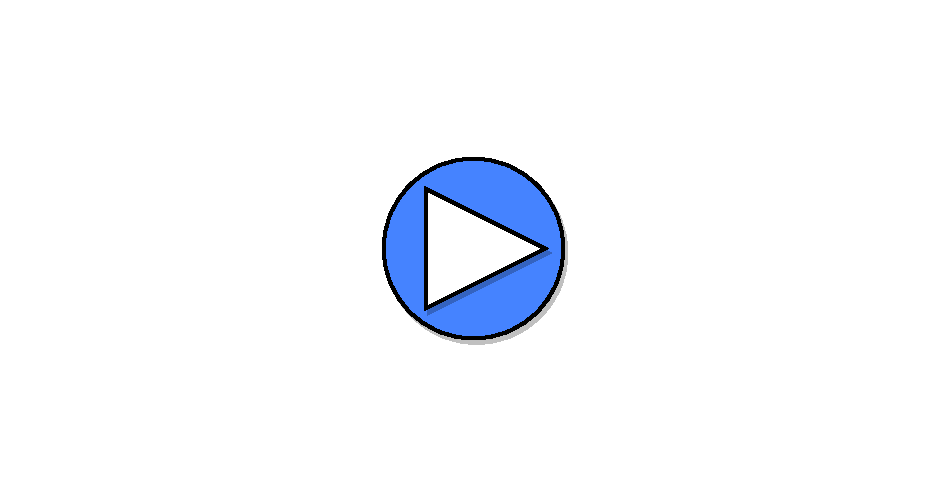
\includegraphics[width=1.08\textwidth]{playbutton.pdf}}{loginOpen.mkv}
}
\end{center}
\end{frame}

%-------------------------------------

\begin{frame}
	\frametitle{Generate and evaluate password}
	\begin{center}
	\vspace{-0.4cm}
	\makebox[0pt]{ %no left margin
		\movie[
		  width=1.03\textwidth,
		  height=0.72\textwidth, 
		  showcontrols,
		  poster
		] 
		{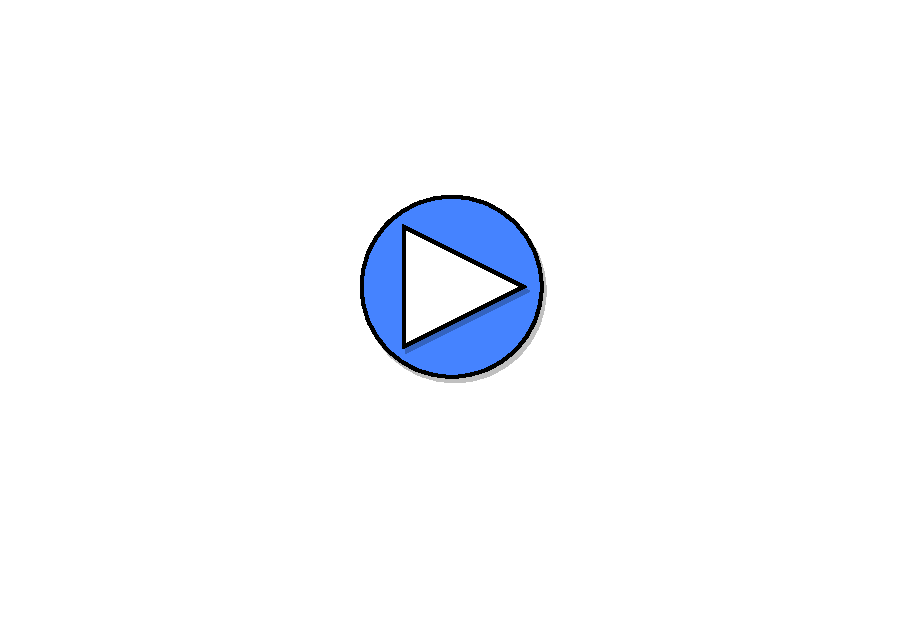
\includegraphics[width=1.03\textwidth]{playbutton2.pdf}}{add.mkv}
	}
	\end{center}
\end{frame}

\section{Conclusions}
\begin{frame}
	\frametitle{Conclusions}
	\begin{itemize}
		\setlength\itemsep{10pt}
		\item<1-> The SEcube™ is perfect for this type of application as it offers both reliability and simplicity to use.
		\item<2-> In any password manager it is important to suggest random passwords and to check their strength
		\item<3-> All the used libraries in this project are open source, proving it is possible to achieve a high level of security with the use of open software and hardware tools. 
		\item<4-> The developed application still lacks some features in order to be considered a truly commercial product.
	
	\end{itemize}
\end{frame}

\section{Future Work}
\begin{frame}
	\frametitle{Future Work}
	{
	\setbeamercolor{block title}{use=structure,bg=MidnightBlue,          fg=white}
	\setbeamercolor{block body} {use=structure,bg=MidnightBlue!10!white, fg=black,}
  \fontsize{14pt}{14}\selectfont

	
  \vspace{-0.3cm}	
	  
	\begin{block}<2->{Web Browse Integration}
  \setbeamercolor*{item}{fg=MidnightBlue}
		\begin{itemize}
		  \item Port the entire Application to a web browser complement.
			\item Web browser complement that "talks" with the SEcubeWallet
			\item Use keyboard emulation to Auto Fill forms
		\end{itemize}
	\end{block}

	\vspace{-0.1cm}	

	\begin{block}<3->{More than static passwords}
	\setbeamercolor*{item}{fg=MidnightBlue}
		\begin{itemize}
			\item One Time Passwords
			\item FIDO U2F
		\end{itemize}
	\end{block}
	
	\vspace{-0.1cm}	
	
	\begin{block}<4->{Android}
	\setbeamercolor*{item}{fg=MidnightBlue}
		\begin{itemize}
			\item Use a SEcube™ phone device
			\item Port SEcube™ host-side libraries to android
			\item Port Qt application to android
		\end{itemize}
	\end{block}	
	}
	
\end{frame}


\end{document}